\section{研究内容及创新点}
\label{sec:intro:work}

\subsection{本文主要内容}
\label{sec:intro:work:mainwork}

随着VoLTE应用范围的不断扩大,研究在VoLTE环境下的时间隐通道构建方案,可以扩充时间隐通道的构建方法,也进一步扩展对VoLTE音视频通话特征的研究。本文主要研究在VoLTE视频通话场景下,通过主动丢包的方式,构建鲁棒的时间隐通道。主要包括三个研究点,分别是VoLTE时间隐通道检测方法研究,基于Zigzag映射矩阵的时间隐通道构建方法研究,以及基于多重校验的时间隐通道构建方法研究。各部分之间的关联关系及研究指标如图\nref{fig:1:contents}。

\insertFigure{
	\begin{figure}
		\centering
        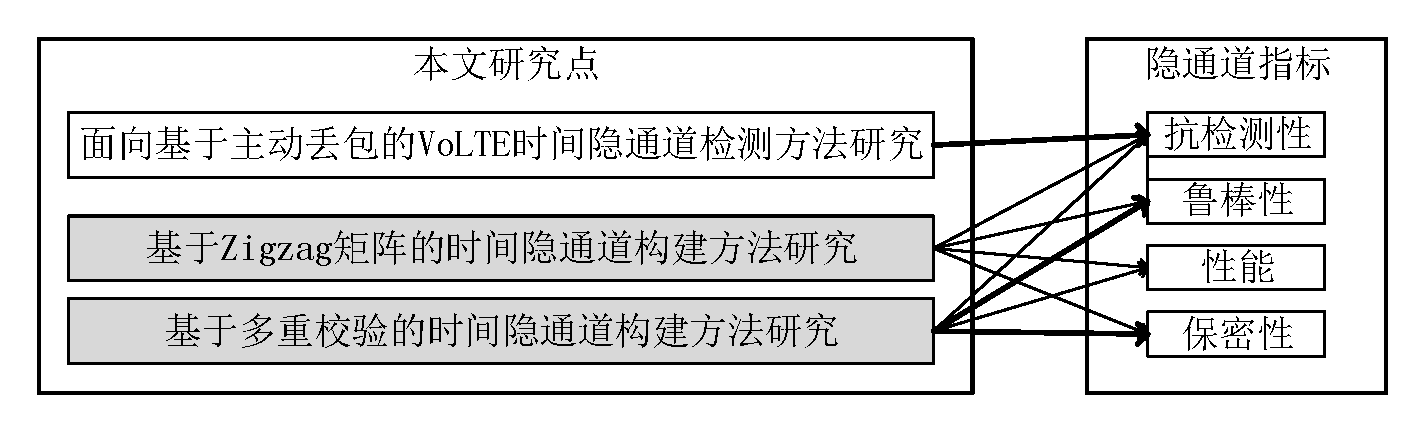
\includegraphics[width=0.75\textwidth]{chapters/chapter1/figures/struct.pdf}
        \caption{本文各研究点之间的关系}\label{fig:1:contents}
	\end{figure}
}

%背景介绍了什么
背景及相关工作部分,主要介绍了本论文主要工作的一些研究基础,以及国内外的研究现状。内容包括对VoLTE音视频传输方案的分析,分析了实际商用中VoLTE的数据产生、处理、传输、呈现流程,并分析了音视频在流程上的差异。对现有时间隐通道构造方案的分析,涵盖了以太网中的构造方案、移动互联网下的构造方案,以及有效的鲁棒性策略。通过分析VoLTE传输协议,研究丢包带来的影响,并充分利用协议中的随机字段,提高保密性。抗检测能力是时间隐通道的一个重要指标,通过研究现有的时间隐通道检测方法,针对该时间隐通道构建方法,选择可用的检测方法。

%检测方法介绍了什么
VoLTE时间隐通道检测方法研究,主要研究在VoLTE场景下,如何有效检测基于主动丢包的时间隐通道。为筛选有效的检测方法,首先对VoLTE通话抓包结果进行分析,由丢包率、IPD、突发丢包长度及丢包随机性几个方面分别展开。根据特征分析结果,提出了一组基于统计分析的时间隐通道检测方法,包含不同维度的多种检测方式。最后,通过模拟的方式,对这些方法进行模拟测试,判断是否具有显著效果。

%Zigzag方法说了什么
基于Zigzag映射矩阵的时间隐通道构建方法,研究利用Zigzag矩阵作为码字与符号关系的映射矩阵,并添加冗余校验信息,在抗检测性、鲁棒性及传输性能之间实现均衡。为了清楚地介绍该研究方法,按照研究背景、构造方法及实验结果及评估的顺序,对该方法的研究基础、架构设计、调制解调方法及实验测试结果分别进行介绍。经过实验测试证明,通过调整传输参数,该时间隐通道构建方法各方面结果良好。

%多重校验方法说了什么
基于多重校验的时间隐通道构建方法,重点研究如何进一步降低误码率,提高传输可靠性。在该时间隐通道方法中,设计了包括码字间校验、码字自校验以及符号校验三级校验模式,结合对连续丢包噪声具有抑制作用的映射矩阵,显著提高了传输鲁棒性,降低了误码率水平。该部分首先从研究背景基础开始,首先介绍该方法的设计架构,然后针对核心的鲁棒性鲁棒性方法逐层展开,最后进行实验测试与对比。实验结果表明,该时间隐通道的误码率水平较之前方案有了大幅度提升。

%以上各部分是怎样在逻辑上串起来的
背景及相关工作的介绍,分析出在VoLTE视频通话场景下,通过主动丢包的方式构建时间隐通道是可行的。与此同时,现有的检测方法及鲁棒性方法,无法有效覆盖这种隐通道构造模式。VoLTE时间隐通道检测方法研究,着重解决如何检测采用主动丢包的时间隐通道,同时也为接下来提出的构建方案提供检测依据。最后,两种不同的时间隐通道构建方法,分别从不同的方式,填补鲁棒性方面的构建需求,并通过实验进行验证。

\subsection{本文主要创新点}
\label{sec:intro:work:inno}

本文的研究重点,是在VoLTE场景下,通过主动丢包方式构建时间隐通道的方法,以及抗检测性评估方式。主要的创新点包括以下几点:

\begin{enumerate}
    \item 提出了一种VoLTE下时间隐通道检测方法,针对基于主动丢包的构建方法。该方法以统计分析为基础,综合多种量化评估方法,结合IPD及丢包特征两个维度进行检测判别。传统的时间隐通道检测方法,主要基于IPD分布特征进行检测识别,对基于主动丢包的时间隐通道来说,判别效果不够全面。本方法完善了时间隐通道的检测方式,经过实验测试,该时间隐通道检测方法有效可行。
    \item 提出了一种基于Zigzag映射矩阵的时间隐通道构建方法,该方法的核心,是隐通道的编码及调制过程,在编码过程中添加CRC校验信息,利用Zigzag矩阵完成码字到符号的转换,最后添加随机偏移量得到要丢弃的数据包序号。该方法以简单高效的方式,以轻量级校验模式,在保证传输性能的同时,降低计算复杂度保证鲁棒性,适用于容许一定误码率的应用场景。
    \item 提出了一种基于多重校验的时间隐通道构造方法,重点研究如何通过逐级校验的方式,降低噪声对时间隐通道的干扰,提高噪声干扰下的鲁棒性。该方法的核心,是在不同的处理阶段引入相互独立的校验方式,在解调过程中逐级剔除噪声干扰,还原概率最高的隐蔽消息。此外,通过引入可调映射矩阵,将连续丢包事件分散到多个组,减小每组的噪声强度,降低误码率水平。
\end{enumerate}

\subsection{本文组织结构}
\label{sec:intro:work:struct}

全文共分五章,文章的组织结构如下:
\begin{itemize}
    \item 第1章,对本文的研究领域及主要内容进行介绍
    \item 第2章,本文中涉及到的研究背景,及国内外相关工作的介绍。包含当前研究工作的基础介绍,当前隐通道构建及检测方面的研究成果,以及时间隐通道应当满足的基本要求。
    \item 第3章,介绍VoLTE下时间隐通道检测方法,结合当前成熟的检测方法,在IPD检测的基础上,添加对丢包特征统计的检测。监测维度涵盖了基于统计曲线的检测、基于熵的检测及基于相对距离的检测方法,能够对基于主动丢包的时间隐通道进行有效识别。该检测方法,也是本文两种时间隐通道构建方法抗检测能力的评估参照。
    \item 第4章,介绍基于Zigzag映射矩阵的时间隐通道构建方法,由研究背景开始,首先介绍构建方法的设计方案,然后通过实验,对隐通道的各项指标进行评估。
    \item 第5章,介绍基于多重校验的时间隐通道构建方法,首先对方法背景进行介绍,然后对时间隐通道的整体流程进行展开,接下来对关键的鲁棒性方案设计逐级展开分析,最后分析实验结果及指标。
\end{itemize}